\chapter{Introduction}

WORK IN PROGRESS

This template 

when there exists an author with last name prefix of 'van', use the \textbackslash VAN command , and follow it up with a \textasciitilde (see reference for example)


\citet*{Allen2002}

\citet*{Bettini2021}

\citet*{Eitelberg2020}

\citet*{Sinnige2020}

\citet*{Herrez2016}


\chapter{Examples}

\section{Tables}

\subsection{tabularx}

\begingroup
\renewcommand\tabularxcolumn[1]{m{#1}} % https://latex.org/forum/viewtopic.php?t=32433

\begin{minipage}[t]{0.48\textwidth}
\begin{table}[H]
    \centering
    \caption{Fuselage geometry \cite[Tab.~4]{Bettini2021}}
    \label{tab:fuselage_geom}
    {\footnotesize
    \begin{tabularx}{\textwidth}[t]{X|rl} \toprule
        \multicolumn{1}{c|}{\textbf{Parameter}} &
        \multicolumn{2}{c}{\textbf{Value}}                  \\ \midrule
        Length          & 1.342     & \si{\meter}           \\
        Diameter        & 0.140     & \si{\meter}           \\
        Volume          & 0.0160632 & \si{\meter\cubed}     \\
        Volume of aft support strut (estimate)  & 0.0004491    & \si{\meter\cubed}  \\
        Volume of wing support struts (estimate for both struts together)                                & 0.0035296   & \si{\meter\cubed} \\ \bottomrule
    \end{tabularx}
    }
\end{table}
\end{minipage}
\hfill
\begin{minipage}[t]{0.48\textwidth}
\begin{table}[H]
    \centering
    \caption{Propeller geometry \cite[Tab.~8]{Bettini2021}}
    \label{tab:prop_geom}
    {\footnotesize
    \begin{tabularx}{\textwidth}[t]{X|rl} \toprule
        \multicolumn{1}{c|}{\textbf{Parameter}}         &
        \multicolumn{2}{c}{\textbf{Value}}                              \\ \midrule
        Number of blades            & 6                 &               \\
        Diameter                    & 0.2032            & \si{\meter}   \\
        Pitch angle at $r/R = 0.7$  & 45                & deg           \\
        Rotation direction (from rear)  & CW    & 2x \\
                                        & CCW   & 1x \\ \bottomrule 
    \end{tabularx}
    }
\end{table}
\end{minipage}

\begin{table}[H]
\caption{Wing geometry \cite[Tab.~5]{Bettini2021}}
\label{tab:wing_geom}
    \begin{subtable}[t]{0.48\textwidth}
    \centering
    {\footnotesize
    \begin{tabularx}{\textwidth}[t]{X|rl} \toprule
        \multicolumn{1}{c|}{\textbf{Parameter}}         &
        \multicolumn{2}{c}{\textbf{Value}}                          \\ \midrule
        Span                    & 1.397     & \si{\meter}           \\
        Area                    & 0.2172    & \si{\meter\squared}   \\
        Mean aerodynamic chord  & 0.165     & \si{\meter}           \\
        Aspect ratio            & 8.98      &                       \\
        Taper ratio             & 0.40      &                       \\
        Sweep angle at $0.25c$  & 0         & deg                   \\
        Incidence angle         & 0         & deg                   \\
        Dihedral angle          & 4         & deg                   \\
        Twist                   & 2         & deg                   \\ \bottomrule
    \end{tabularx}
    }
    \end{subtable}
    \hfill
    \begin{subtable}[t]{0.48\textwidth}
    \centering
    {\footnotesize
    \begin{tabularx}{\textwidth}[t]{X|rl} \toprule
        \multicolumn{1}{c|}{\textbf{Parameter}}         &
        \multicolumn{2}{c}{\textbf{Value}}                                                  \\ \midrule
        Airfoil (constant over span)        & DU 96-150                 &                   \\
        Aileron span                        & 0.197                     & \si{\meter}       \\
        Aileron spanwise position           & 0.71 < y/(b/2) < 0.99     &                   \\
        Aileron chord                       & 0.029                     & \si{\meter}       \\ 
        Flap span (per side)                & 0.369                     & \si{\meter}       \\
        Flap chord                          & 0.060                     & \si{\meter}       \\
        Wing $0.25c$ from fuselage nose     & 0.680                     & \si{\meter}       \\
        Volume                              & 0.0030229                 & \si{\meter\cubed} \\ \bottomrule
    \end{tabularx}
    }
    \end{subtable}
\end{table}

\endgroup


\section{Graphs}

\subsection{subfigures}
\begin{figure}[H]
    \centering
    \begin{subfigure}[t]{0.48\textwidth}
        \centering
        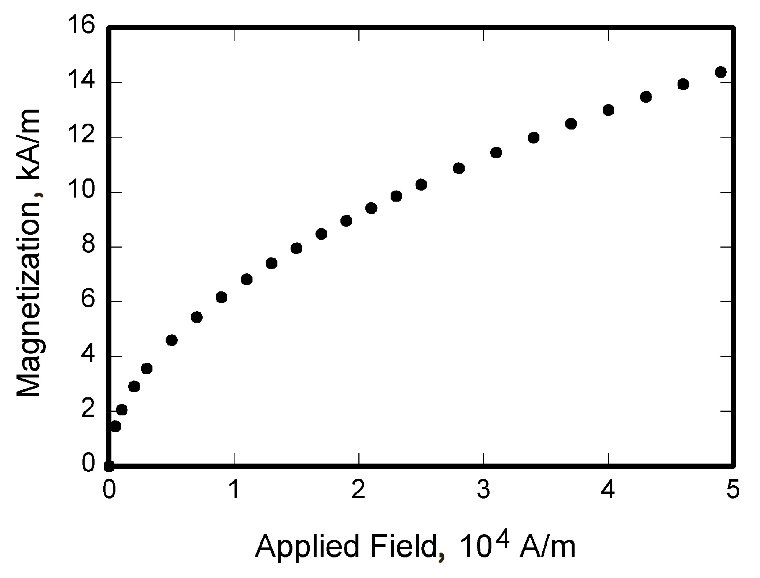
\includegraphics[width=1.0\textwidth]{Images/graph.jpg}
        \caption{graph 1}
        \label{subfig:graph1}
    \end{subfigure}
    \hfill
    \begin{subfigure}[t]{0.48\textwidth}
        \centering
        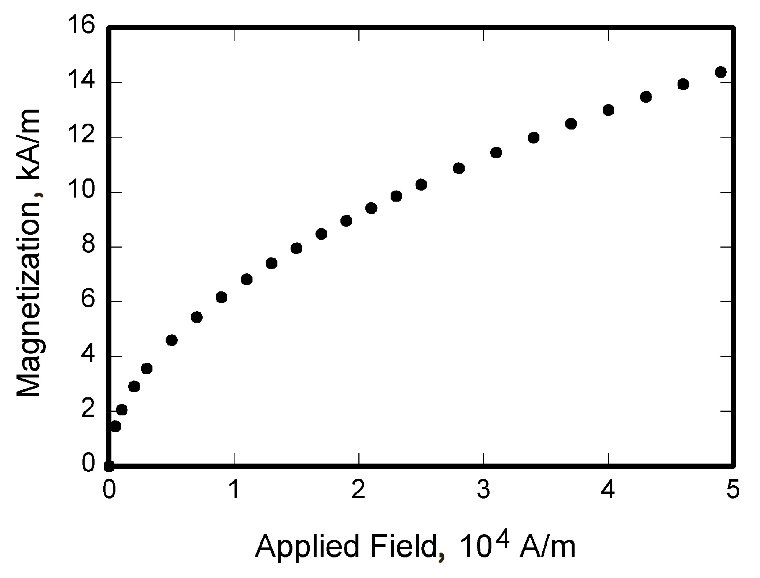
\includegraphics[width=1.0\textwidth]{Images/graph.jpg}
        \caption{graph 2}
        \label{subfig:graph2}
    \end{subfigure}
    \bigskip
    \begin{subfigure}[t]{0.48\textwidth}
        \centering
        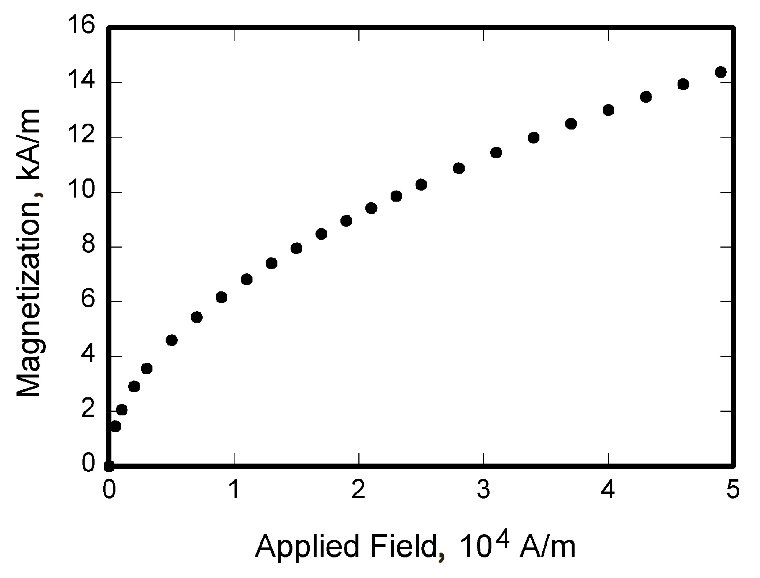
\includegraphics[width=1.0\textwidth]{Images/graph.jpg}
        \caption{graph 3 help help help help help help help help help help help help help}
        \label{subfig:graph3}
    \end{subfigure}
    \hfill
    \begin{subfigure}[t]{0.48\textwidth}
        \centering
        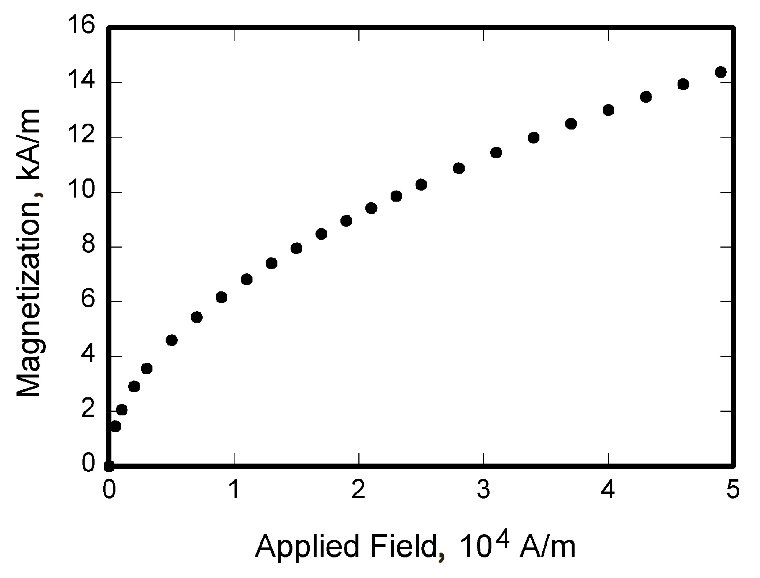
\includegraphics[width=1.0\textwidth]{Images/graph.jpg}
        \caption{graph 4}
        \label{subfig:graph4}
    \end{subfigure}
    \caption{graphs (subfigures)}
    \label{fig:graph_subfigures}
\end{figure}

\subsection{Continued float}
\begin{figure}[H]
    \centering
    \begin{subfigure}[t]{0.48\textwidth}
        \centering
        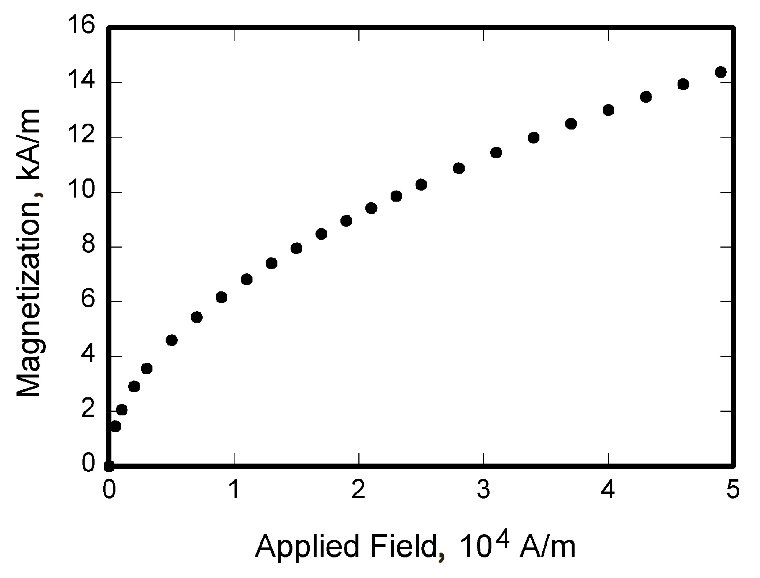
\includegraphics[width=1.0\textwidth]{Images/graph.jpg}
        \caption{graph 5}
        \label{subfig:graph5}
    \end{subfigure}
    \hfill
    \begin{subfigure}[t]{0.48\textwidth}
        \centering
        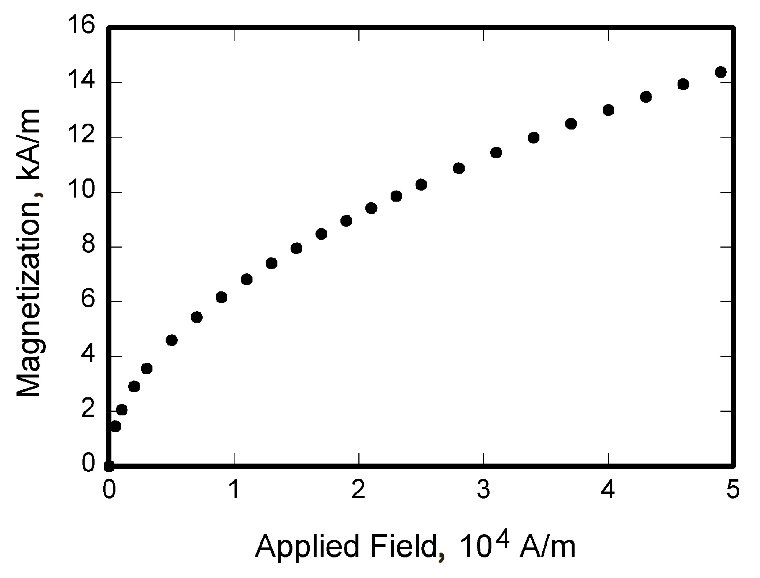
\includegraphics[width=1.0\textwidth]{Images/graph.jpg}
        \caption{graph 6}
        \label{subfig:graph6}
    \end{subfigure}
\end{figure}%
\begin{figure}[H]\ContinuedFloat
    \begin{subfigure}[t]{0.48\textwidth}
        \centering
        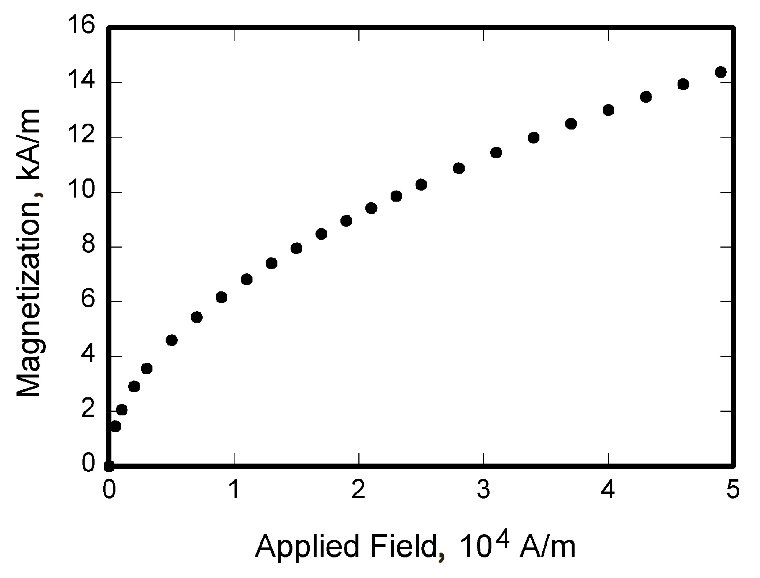
\includegraphics[width=1.0\textwidth]{Images/graph.jpg}
        \caption{graph 7}
        \label{subfig:graph7}
    \end{subfigure}
    \hfill
    \begin{subfigure}[t]{0.48\textwidth}
        \centering
        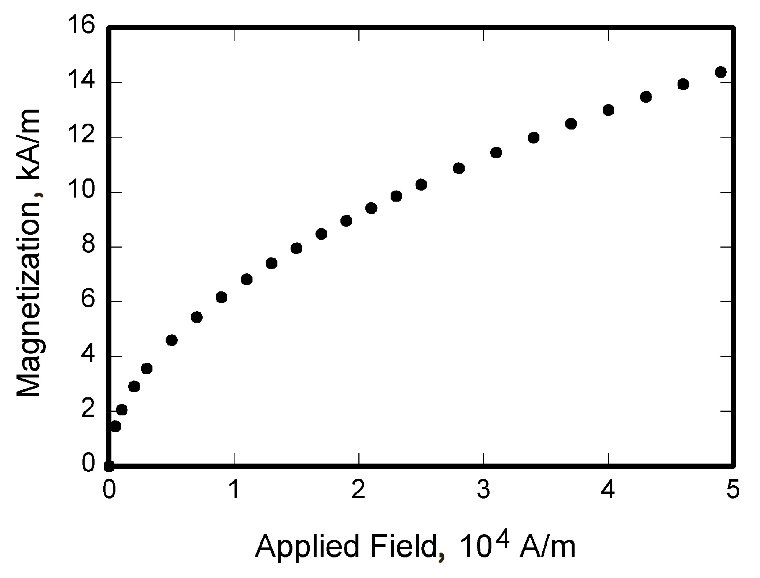
\includegraphics[width=1.0\textwidth]{Images/graph.jpg}
        \caption{graph 8}
        \label{subfig:graph8}
    \end{subfigure}
    \caption{graphs (continued float)}
    \label{fig:graph_contfloat}
\end{figure}

\subsubsection{Aligned graphs}

\begin{figure}[H]
\begin{tabular}{@{}p{0.485\textwidth}p{0.485\textwidth}@{}}
    \raisebox{-\height}{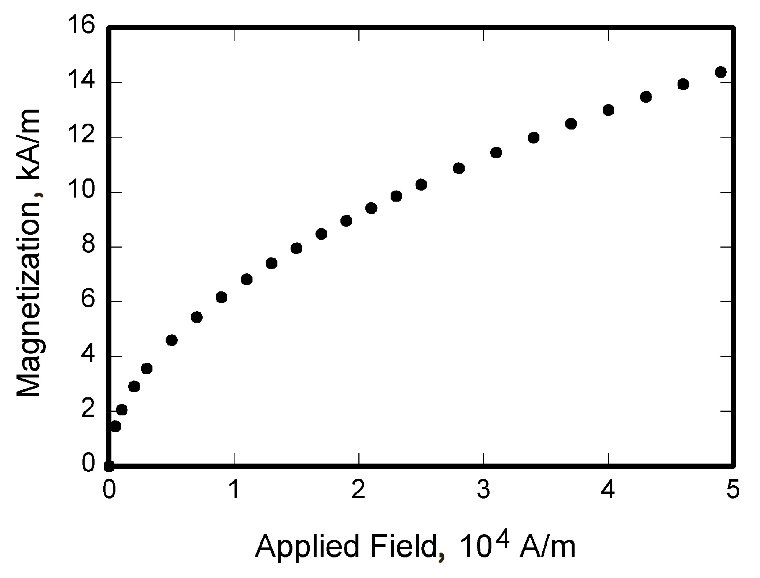
\includegraphics[width=1.0\linewidth]{Images/graph.jpg}}&
    \raisebox{-\height}{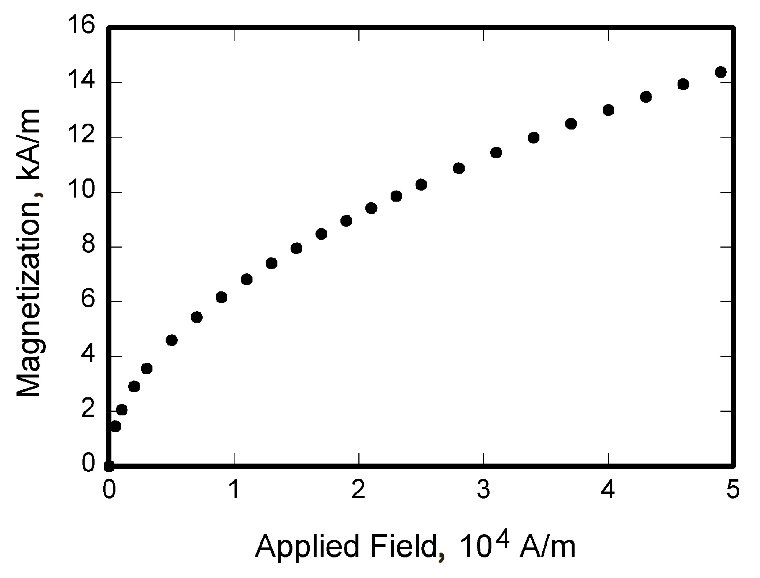
\includegraphics[width=1.0\linewidth]{Images/graph.jpg}}\\
    \caption{graph}\label{fig:graph9}&
    \caption{graph graph graph graph graph graph graph graph graph graph graph graph graph graph graph graph}\label{fig:graph10}
\end{tabular}
\end{figure}

\subsubsection{Aligned repeated graphs}
\begin{figure}[H]
\begin{tabular}{@{}p{0.485\textwidth}p{0.485\textwidth}@{}}
    \raisebox{-\height}{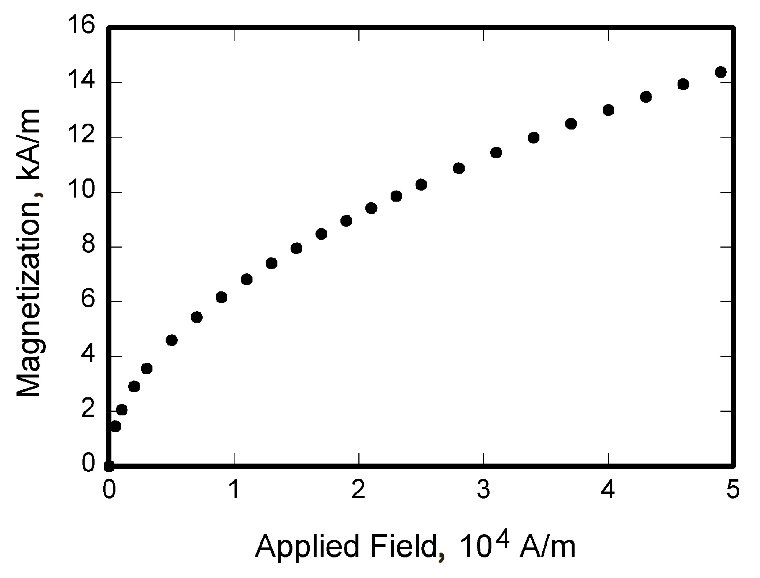
\includegraphics[width=1.0\linewidth]{Images/graph.jpg}}&
    \raisebox{-\height}{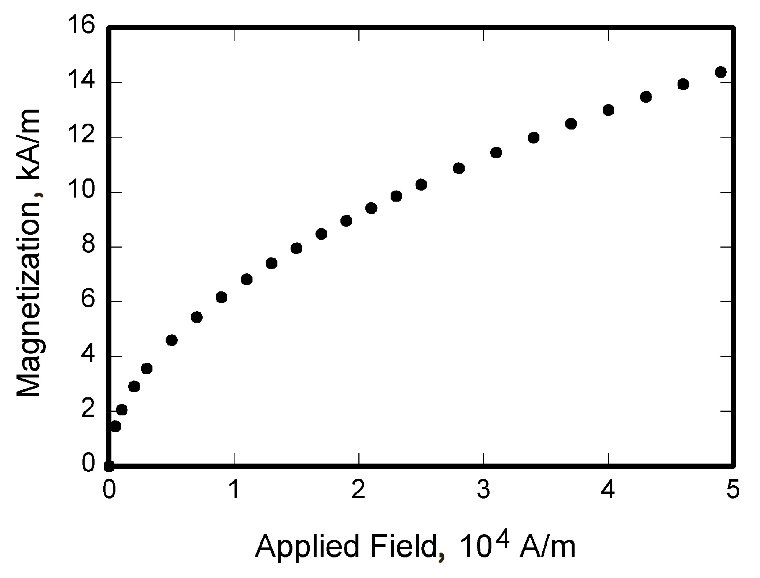
\includegraphics[width=1.0\linewidth]{Images/graph.jpg}}\\
    \repeatcaption{fig:graph9}{graph}&
    \repeatcaption{fig:graph10}{graph graph graph graph graph graph graph graph graph graph graph graph graph graph graph graph }
\end{tabular}
\end{figure}